\documentclass[11pt]{article}

%============================= PACKAGES =================================
\usepackage[margin=1in]{geometry}
\usepackage{amsmath}
\usepackage{amssymb}
\usepackage{amsthm}
\usepackage{mathtools}
\usepackage{bm}
\usepackage{array}
\usepackage{tikz}
\usetikzlibrary{decorations.pathmorphing,arrows.meta,calc,positioning}
\usepackage{booktabs}
\usepackage{enumitem}
\usepackage{xcolor}
\usepackage{titlesec}
\usepackage{fancyhdr}
\usepackage[colorlinks=true,linkcolor=shpblue,citecolor=shpblue,urlcolor=shpblue]{hyperref}

%============================= COLORS ====================================
\definecolor{shpblue}{RGB}{21,67,120}
\definecolor{shpred}{RGB}{150,30,30}
\definecolor{shpgray}{RGB}{95,95,95}

%============================= SECTION STYLE ==============================
\titleformat{\section}{\normalfont\Large\bfseries\color{shpblue}}{\thesection}{1em}{}
\titleformat{\subsection}{\normalfont\large\bfseries\color{shpblue!85!black}}{\thesubsection}{1em}{}
\titleformat{\subsubsection}{\normalfont\normalsize\bfseries\color{shpblue!70!black}}{\thesubsubsection}{1em}{}

%============================= HEADER/FOOTER ==============================
\pagestyle{fancy}
\fancyhf{}
\fancyhead[L]{\small\textit{Off-Shell Dynamics and Extended Objects}}
\fancyhead[R]{\small\thepage}
\renewcommand{\headrulewidth}{0.4pt}

%============================= THEOREM-LIKE ENVIRONMENTS ==================
\newtheorem{remark}{Remark}[section]

%============================= MISC ========================================
\setlength{\parskip}{2pt}
\setcounter{secnumdepth}{3}
\setcounter{tocdepth}{2}

\newcommand{\eqn}[1]{Eq.~\eqref{#1}}
\newcommand{\eqns}[2]{Eqs.~\eqref{#1}--\eqref{#2}}

\title{\textbf{Off-Shell Relativistic Dynamics and Space-Time Extended Objects:\\[2pt]
\large Strings and Branes in the Stueckelberg--Horwitz--Piron Framework}}

\author{Author Name$^{1}$\\
\small $^1$Affiliation, Department, Institution\\
\small \texttt{author@institution.edu}}
% NOTE TO USER: replace the author/affiliation block above with your own details.

\date{\today}

\begin{document}
\sloppy

\maketitle

\begin{abstract}
\noindent
The Stueckelberg--Horwitz--Piron (SHP) formalism replaces the single relativistic
worldline parametrized implicitly by coordinate time with a manifestly covariant
mechanics in which spacetime events $x^\mu(\tau)$ evolve with respect to a genuine
fifth, Poincar\'e-invariant parameter $\tau$, while the four-momentum -- and hence
the particle's mass -- is generically \emph{off} the mass shell and becomes a
dynamical quantity. We review the single-event and many-body SHP formalism, its
associated five-dimensional (``pre-Maxwell'') gauge theory, and then turn to the
paper's central theme: how this off-shell dynamics extends from point particles to
space-time \emph{extended objects}. We give a self-contained account of the explicit
construction, due to Suleymanov, Horwitz and Yahalom, of a relativistic string as
the continuum limit of a closed chain of off-shell events bound by invariant-interval
potentials, including its mode spectrum, its Regge-like mass formula, and its
unusual mode of ``second quantization'' that never introduces negative-norm
oscillators. We compare this Hamiltonian, manifestly-covariant construction with
the reparametrization-invariant Nambu--Goto/Polyakov string, clarify why the SHP
string requires no critical spacetime dimension, and relate the whole programme to
Pavši\v{c}'s independently developed ``unconstrained'' theory of relativistic
$p$-branes, which is built on the same Fock--Stueckelberg notion of an invariant
evolution parameter. Finally, we sketch -- explicitly flagged as an outlook rather
than an established result -- a natural two-parameter generalization of the SHP
string construction toward off-shell membranes, and discuss the open problems this
generalization raises.
\end{abstract}

\noindent\textbf{Keywords:} Stueckelberg--Horwitz--Piron theory; off-shell dynamics;
relativistic quantum mechanics; invariant evolution parameter; extended objects;
relativistic strings; $p$-branes; pre-Maxwell electrodynamics; Regge trajectories.

\vspace{4pt}
\hrule
\vspace{4pt}

{\small\tableofcontents}

\clearpage

%############################################################################
\section{Introduction}
%############################################################################

\subsection{The problem of time in relativistic quantum theory}

Non-relativistic quantum mechanics rests on a sharp distinction between the
Newtonian time $t$, an external, universal parameter of evolution, and the
position operator $\hat{\bm x}$, which is a dynamical variable with its own
spectral resolution. Special relativity spoils this distinction: under a Lorentz
transformation $t$ mixes with the spatial coordinates, so it can no longer
consistently be held external to the dynamics while $\bm x$ is treated as an
operator. The two standard routes out of this difficulty -- the Klein--Gordon and
Dirac equations -- restore covariance by promoting $x^0=ct$ to an operator on the
same footing as $\bm x$, but at a price: the Klein--Gordon current's time
component is not positive-definite, and although the Dirac current is positive,
Newton and Wigner showed that the associated localized states are non-local in a
precise sense, spreading over a region of order the Compton wavelength
$1/m$ \cite{NewtonWigner1949}. A further, largely independent obstruction
appears as soon as one tries to describe \emph{several} mutually interacting
relativistic particles in Hamiltonian form: Currie, Jordan and Sudarshan proved
that manifestly covariant canonical position variables for two or more particles,
each generating its own time translations, are compatible with nontrivial
interaction only in a very restricted sense -- the ``no-interaction theorem''
\cite{CurrieJordanSudarshan1963}. Any framework that hopes to treat interacting
relativistic many-body systems in a genuinely Hamiltonian way must therefore
depart from the na\"ive idea that each particle carries its own proper time as
the evolution parameter of the whole system.

\subsection{Fock, Stueckelberg, and the invariant evolution parameter}

The resolution adopted in this paper's subject traces back to Fock
\cite{Fock1937} and, in its modern form, to Stueckelberg
\cite{Stueckelberg1941a,Stueckelberg1941b,Stueckelberg1942}, who introduced a
\emph{fifth}, Lorentz-invariant parameter $\tau$ -- distinct from, and external
to, the coordinate $x^0=ct$ -- with respect to which the spacetime event
$x^\mu(\tau)$ evolves. Stueckelberg's original motivation was to give a
manifestly covariant, single-particle description of pair creation and
annihilation: because $x^0(\tau)$ need not increase monotonically with $\tau$,
a single worldline that first moves forward and then backward in coordinate time
can represent, in the usual Feynman--Stueckelberg reading, a particle and its
antiparticle joined at a pair-creation or annihilation vertex. Since $\tau$, not
$t$, is now the true evolution parameter, energy and momentum become independent
of one another along the trajectory: the particle's mass is no longer a fixed
external label but an \emph{observable}, generically varying as the system
evolves. This is the sense in which the theory is \emph{off-shell}: the
four-momentum need not, instant by instant, satisfy the mass-shell condition
$p^\mu p_\mu=-m_0^2c^2$ for any fixed $m_0$.

Horwitz and Piron generalized Stueckelberg's single-particle idea to a
consistent many-body theory by making a further conceptual commitment: $\tau$ is
taken to be \emph{universal}, playing for the relativistic many-body system
exactly the role Newtonian time plays non-relativistically
\cite{HorwitzPiron1973}. Because all particles of an interacting system share
the same $\tau$, manifestly covariant potentials that depend on the
spacelike-separated positions of two or more particles \emph{at equal $\tau$}
can be written down consistently, sidestepping the no-interaction theorem, which
applies to theories built instead from $N$ separate proper times. This
Stueckelberg--Horwitz--Piron (SHP) theory, together with its extensions, is
reviewed in detail in Horwitz's monograph \cite{Horwitz2015} and is the subject
of a large literature; see also \cite{HorwitzArshanskyElitzur1988} for a
discussion of the distinction between $\tau$ and $t$ and its physical
implications.

\subsection{Why extended objects?}

The question addressed in this paper is what happens to this picture once one
asks not for a single event, or a finite number of mutually interacting events,
but for a \emph{continuum} of them -- a string or a membrane. This question is
independently interesting for at least three reasons.

First, it is a natural completion of the SHP research programme: the many-body
sector of SHP theory already treats an arbitrary finite collection of events
sharing one evolution parameter $\tau$; letting the number of events tend to
infinity while they remain mutually bound is the obvious route to a covariant,
off-shell theory of continuous matter.

Second, it offers a genuinely different notion of ``off-shell'' extended object
from the one familiar in string theory proper. In the covariant quantization of
the Nambu--Goto or Polyakov string, ``off-shell'' string configurations are
those that violate the Virasoro (mass-shell) constraints generated by
worldsheet reparametrization invariance -- essentially gauge artifacts to be
projected out. In the SHP string, by contrast, off-shell-ness is a genuine
additional \emph{dynamical} freedom, exactly as for the point particle: the
mass of the extended object, and indeed the local four-momentum of each piece
of it, need not sit on any fixed shell, and the theory is formulated in a
Hamiltonian, not a constrained/reparametrization-invariant, language from the
outset.

Third, an explicit construction of this kind already exists in the literature
-- due to Suleymanov, Horwitz and Yahalom \cite{SuleymanovHorwitzYahalom2017}
-- and is, to date, the clearest concrete bridge between SHP theory and the
physics of extended objects. Section~\ref{sec:string} of this paper is devoted
to a self-contained account of that construction.

\subsection{Outline}

Sections~\ref{sec:single}--\ref{sec:gauge} review the single-event and
many-body SHP formalism and its associated pre-Maxwell gauge theory, at the
level of detail needed for what follows.
Section~\ref{sec:string} is the technical core of the paper: it develops the
SHP relativistic string as the continuum limit of a covariant chain of
off-shell events, its steady rotating solution, its oscillation spectrum, its
Regge-like mass formula, and its distinctive route to quantization.
Section~\ref{sec:comparison} compares this construction with the standard
Nambu--Goto/Polyakov string. Section~\ref{sec:pavsic} situates it relative to
Pavši\v{c}'s independently developed unconstrained theory of relativistic
$p$-branes, which shares the same Stueckelberg-type philosophy but was built on
a different, more geometric, route. Section~\ref{sec:outlook} sketches --
explicitly as an outlook, not an established result -- how the SHP string
construction might be generalized to membranes, and what new difficulties
arise. Section~\ref{sec:discussion} discusses the overall picture and
Section~\ref{sec:conclusion} concludes.


%############################################################################
\section{The SHP Formalism for a Single Event}
\label{sec:single}
%############################################################################

\subsection{Classical mechanics}

Throughout we use the metric signature $\eta_{\mu\nu}=\mathrm{diag}(-1,+1,+1,+1)$,
$\mu,\nu=0,1,2,3$, and write $x^\mu=(ct,\bm x)$, $p^\mu=(E/c,\bm p)$ for a single
spacetime event. The central postulate of SHP theory is the existence of a
manifestly covariant, Lorentz-scalar Hamiltonian function $K(x,p,\tau)$ that
generates the evolution of the event in the invariant parameter $\tau$ through
Hamilton-type equations,
\begin{equation}
\frac{dx^\mu}{d\tau}=\frac{\partial K}{\partial p_\mu}\,,\qquad
\frac{dp^\mu}{d\tau}=-\frac{\partial K}{\partial x_\mu}\,,
\label{eq:hameqs}
\end{equation}
with canonical Poisson bracket $\{x^\mu,p^\nu\}=\eta^{\mu\nu}$. As $\tau$ runs
over the reals, $x^\mu(\tau)$ traces out the particle's worldline. Unlike the
proper-time parametrization of ordinary relativistic mechanics, $\tau$ here is
\emph{not} defined kinematically in terms of the trajectory; it is postulated
from the outset as an independent, external parameter, on exactly the same
logical footing as $t$ in non-relativistic mechanics.

For a free event one may take
\begin{equation}
K_0=\frac{p^\mu p_\mu}{2M}=\frac{\bm p^2-E^2/c^2}{2M}\,,
\label{eq:K0}
\end{equation}
where $M$ is an intrinsic parameter of the particle with dimensions of mass,
fixed once and for all -- it is \emph{not} to be confused with the
\emph{observed} or \emph{dynamical} mass $m$, defined by
$p^\mu p_\mu\equiv -m^2c^2$, which is in general a function of $\tau$. Because
$K$ has no explicit $\tau$-dependence, it is itself a constant of the motion,
\begin{equation}
\frac{dK}{d\tau}=\frac{\partial K}{\partial x^\mu}\frac{\partial K}{\partial p_\mu}
-\frac{\partial K}{\partial p_\mu}\frac{\partial K}{\partial x^\mu}=0\,,
\label{eq:Kconserved}
\end{equation}
by direct substitution of \eqn{eq:hameqs} -- this is simply the statement that
the Poisson bracket of $K$ with itself vanishes. For the free Hamiltonian
\eqref{eq:K0}, $\partial K_0/\partial x^\mu=0$ identically, so $p^\mu$ itself,
not merely $K_0$, is separately conserved along a free trajectory: a free event
remains forever on whatever mass shell $-m^2c^2=p^\mu p_\mu$ it started on. This
already shows that ``off-shell'' does not mean ``never on a shell'' -- it means
that $m$ is not fixed \emph{a priori} to a single, universal value for all
histories of a given particle, as it is in the standard on-shell theory;
genuine $\tau$-dependence of $m^2$ requires interaction.

Including an invariant interaction, $K=p^\mu p_\mu/(2M)+V(x)$, one finds from
\eqref{eq:hameqs} that $dx^\mu/d\tau=p^\mu/M$, so that $K$ may equally be
written in terms of four-velocities as
\begin{equation}
K=\tfrac{1}{2}M\,\dot x_\mu \dot x^\mu+V(x)\,,\qquad \dot x^\mu\equiv \frac{dx^\mu}{d\tau}\,,
\label{eq:Kvelocity}
\end{equation}
and, separating time and space components,
$dt/d\tau=E/(Mc^2)$, $d\bm x/d\tau=\bm p/M$, which combine to give the familiar
relation $d\bm x/dt=\bm p c^2/E$. The coordinates $(t,\bm x)$ that appear here
are to be read as the outcome of a measurement -- a detected signal generated
by the event at parameter value $\tau$ -- so that $t$ plays the role of a
laboratory clock reading rather than of the evolution parameter itself.

Because $K$ has no explicit $\tau$-dependence it remains a constant of the
motion even in the interacting case; for a trajectory normalized so that this
conserved value equals $-Mc^2/2$ (as for a particle that is asymptotically on
the $M$-shell in the absence of interaction), \eqref{eq:Kvelocity} together with
$p^\mu p_\mu=-m^2c^2$ gives
\begin{equation}
m^2=M^2+\frac{2M}{c^2}\,V(x)\,,
\label{eq:massformula}
\end{equation}
which coincides with $M$ exactly when $V=0$ or in the non-relativistic limit
$c\to\infty$. One can further show that $\tau$ coincides with the particle's
own proper time precisely when $m=M$
\cite{HorwitzPiron1973,Horwitz2015}: the ``mass shell,'' in this sense, is a
special, not a generic, condition.

\begin{remark}[On the meaning of ``off-shell'']
In SHP theory, off-shell dynamics is not a statement that relativistic
kinematics is violated; $p^\mu p_\mu=-m^2c^2$ holds at every instant $\tau$,
exactly as in the on-shell theory. What is relaxed is the assumption that $m$
is a fixed constant characterizing the particle species for all time; instead
$m^2(\tau)$ is a genuine dynamical variable, determined by \eqref{eq:massformula}
or its interacting/many-body generalizations, that may fluctuate during an
interaction and relax back toward $M$ once the interaction switches off.
\end{remark}

\subsection{Quantization}

Quantization proceeds by promoting $x^\mu$ and $p^\mu$ to self-adjoint
operators on $L^2(\mathbb{R}^4)$ satisfying the covariant commutation relations
\begin{equation}
[x^\mu,p^\nu]=i\hbar\,\eta^{\mu\nu}\,,
\label{eq:commutator}
\end{equation}
so that $p^0=E/c$, with spectrum $(-\infty,\infty)$, generates translations in
$t$ exactly as $\bm p$ generates translations in $\bm x$. States are described
by a wavefunction $\psi_\tau(x)$ evolving according to the
Stueckelberg--Schr\"odinger equation
\begin{equation}
i\hbar\,\frac{\partial \psi_\tau(x)}{\partial \tau}=K\,\psi_\tau(x)\,,
\label{eq:stueckschrod}
\end{equation}
a direct relativistic generalization of the ordinary Schr\"odinger equation in
which $K$ replaces the non-relativistic Hamiltonian and $\tau$ replaces $t$.
The quantity $|\psi_\tau(x)|^2$ is interpreted as the probability density,
normalized as $\int d^4x\,|\psi_\tau(x)|^2=1$, for detecting the event at the
spacetime point $x^\mu$ -- that is, for receiving a signal generated by the
particle at historical time $\tau$ in the laboratory region $d^3x$ around
$\bm x$ during the coordinate-time interval $dt$ around $t$. Because $x^\mu$ is
a genuine self-adjoint position operator on $\mathbb{R}^4$ and $|\psi_\tau|^2$
is manifestly positive by construction, this construction sidesteps both the
Klein--Gordon indefinite-density problem and the Newton--Wigner non-locality
obstruction mentioned above.

\subsection{Correlation and the classical/on-shell limit}
\label{sec:correlation}

The observed near-universality of particle masses is recovered in SHP theory
as a dynamical, rather than kinematic, statement. Loosely speaking, for
asymptotic states -- those in the far past or far future of an interaction --
the mass-squared operator becomes sharply peaked (``correlated'') about a
definite value, so that the most probable worldline traced out as $\tau$
evolves approaches an ordinary on-shell relativistic trajectory once the
interaction has switched off; this asymptotic clustering property, together
with the explicit relaxation mechanisms discussed in
Section~\ref{sec:massstability} below, is what allows SHP theory to reduce to
the standard on-shell theory of relativistic particles in the appropriate
limits while retaining genuinely off-shell behavior during interactions
\cite{Horwitz2015,HorwitzPiron1973}.


%############################################################################
\section{Many-Body Theory and the Relative-Motion Problem}
\label{sec:manybody}
%############################################################################

\subsection{The $N$-body Hamiltonian}

The many-body generalization of \eqref{eq:K0}--\eqref{eq:Kvelocity} is
immediate precisely because $\tau$ is universal: for $N$ events
$x_i^\mu(\tau)$, $i=1,\dots,N$, one writes
\begin{equation}
K=\sum_{i=1}^{N}\frac{p_{i\mu}p_i^{\ \mu}}{2M_i}+V(x_1,\dots,x_N)\,,
\label{eq:Kmanybody}
\end{equation}
with Hamilton's equations $\dot x_i^\mu=\partial K/\partial p_{i\mu}=p_i^\mu/M_i$,
$\dot p_i^\mu=-\partial K/\partial x_{i\mu}$, on the unconstrained $8N$-dimensional
phase space spanned by all the $x_i^\mu,p_i^\mu$. Crucially, $V$ may depend on
the positions of two or more particles \emph{at equal $\tau$} without running
afoul of the no-interaction theorem of Currie, Jordan and Sudarshan
\cite{CurrieJordanSudarshan1963}, precisely because that theorem concerns
theories built from $N$ separate, particle-proper-time generators of evolution,
whereas here a single $\tau$-translation generator $K$ governs the whole
system.

\subsection{Two-body relative motion and the restricted Minkowski space}
\label{sec:RMS}

For two events, the natural relativistically invariant interaction depends on
the spacelike interval
\begin{equation}
\rho^2\equiv(x_1-x_2)^\mu(x_1-x_2)_\mu\,,
\label{eq:rho2}
\end{equation}
through a potential $V(\rho)$. Separating center-of-mass and relative
coordinates,
\begin{equation}
P^\mu=p_1^\mu+p_2^\mu,\quad
X^\mu=\frac{M_1x_1^\mu+M_2x_2^\mu}{M_1+M_2},\quad
p^\mu=\frac{M_2p_1^\mu-M_1p_2^\mu}{M_1+M_2},\quad
x^\mu=x_1^\mu-x_2^\mu\,,
\label{eq:cmrelative}
\end{equation}
with reduced mass $m=M_1M_2/(M_1+M_2)$ and total mass $M=M_1+M_2$, one obtains
$K=P^2/2M+p^2/2m+V(\rho)\equiv P^2/2M+K_{\rm rel}$, and the
Stueckelberg--Schr\"odinger equation separates into a free center-of-mass part
and an eigenvalue problem for the relative motion,
\begin{equation}
K_{\rm rel}\,\psi^{(a)}(P,x)=\left(-\frac{\partial^\mu\partial_\mu}{2m}+V(\rho)\right)\psi^{(a)}(P,x)=K_a\,\psi^{(a)}(P,x)\,.
\label{eq:relativeeigen}
\end{equation}
The two-body invariant mass squared is then $s_a\equiv -P_a^2=2M(K_a-K)$.

A subtlety specific to the relativistic problem is the domain of the relative
coordinate $x^\mu$. Arshansky and Horwitz showed that taking the potential to
be supported on the full spacelike region leads to an incorrect spectrum for
the Coulomb-type problem, whereas restricting the domain of support to a
particular $O(2,1)$-invariant sub-region of the spacelike interval -- the
\emph{restricted} (or reduced) \emph{Minkowski space}, RMS, identified earlier
by Zmuidzinas in his study of unitary representations of the Lorentz group on
four-vector manifolds \cite{Zmuidzinas1966} -- reproduces the correct
non-relativistic (Balmer-type) spectrum up to relativistic corrections
\cite{ArshanskyHorwitz1989}. The RMS is conveniently parametrized by
$(\rho,\theta,\phi,\beta)$ through
\begin{equation}
x^0=\rho\sin\theta\sinh\beta,\quad
x^1=\rho\sin\theta\cos\phi\cosh\beta,\quad
x^2=\rho\sin\theta\sin\phi\cosh\beta,\quad
x^3=\rho\cos\theta\,,
\label{eq:RMSparam}
\end{equation}
so that $x^\mu x_\mu=\rho^2$ identically (Appendix~\ref{app:rms}); the
resulting wavefunctions vanish at the boundary of this region, so there is no
tunneling into the timelike domain. Bound-state wavefunctions on the RMS
provide the building block re-used throughout the rest of this paper.

\subsection{The relativistic harmonic oscillator}
\label{sec:oscillator}

Of particular importance for Section~\ref{sec:string} is the relativistic
generalization of the isotropic harmonic oscillator,
\begin{equation}
V(\rho)=\tfrac{1}{2}m\omega^2\rho^2\,,
\label{eq:oscpotential}
\end{equation}
whose eigenvalue problem on the RMS was solved exactly by Arshansky and
Horwitz \cite{ArshanskyHorwitz1989}, giving a discrete spectrum
\begin{equation}
K_{rl}=\hbar\omega\left(l+2r+\tfrac{3}{2}\right)\,,
\label{eq:oscspectrum}
\end{equation}
labeled by a set of four quantum numbers $\lambda=(l,r,p,m)$: an
angular-momentum-type number $l$ and a radial number $r$ entering the energy
directly, associated respectively with Laguerre-type radial functions and
$O(2,1)$-type angular functions on the RMS, together with two further labels
$(p,m)$ that parametrize degeneracy. This eigenvalue problem is, up to
relabeling, identical to the ordinary three-dimensional isotropic quantum
harmonic oscillator problem, whose spectrum $E_{n_rl}=\hbar\omega(2n_r+l+3/2)$
it reproduces in form; the extra, boost-like RMS variable $\beta$ contributes
only to the degeneracy structure, not to the energy itself. From
\eqref{eq:relativeeigen}, this spectrum feeds directly into the composite
system's invariant mass through $s=2M(K_{\rm rel}-K)$, so that internal
oscillator excitations shift the physical mass-squared of the bound system in
discrete steps -- the mechanism re-used, for a continuum of coupled
oscillators, in the derivation of the string mass spectrum in
Section~\ref{sec:regge}.


%############################################################################
\section{Gauge Invariance and the Pre-Maxwell Field}
\label{sec:gauge}
%############################################################################

\subsection{Five compensation fields}

Ordinary electrodynamics arises from demanding invariance of a quantum theory
under local phase transformations that depend on spacetime position. In SHP
theory the wavefunction depends on the additional parameter $\tau$, and there
is no obstruction to letting the local phase also depend on $\tau$:
\begin{equation}
\psi_\tau(x)\ \longrightarrow\ e^{ie\Lambda(x,\tau)}\,\psi_\tau(x)\,.
\label{eq:gaugephase}
\end{equation}
Demanding that the Stueckelberg--Schr\"odinger equation~\eqref{eq:stueckschrod}
retain its form under \eqref{eq:gaugephase} forces the introduction of not
one but \emph{five} compensating gauge fields: the familiar four-vector
potential $a_\mu(x,\tau)$, whose covariant derivative $D_\mu=\partial_\mu+iea_\mu$
absorbs the $x$-dependence of $\Lambda$ exactly as in ordinary electrodynamics,
\emph{and} a fifth, scalar compensation field $a_5(x,\tau)$ that absorbs the
$\tau$-dependence of $\Lambda$ through $D_\tau=\partial_\tau+iea_5$. This
five-field structure -- the ``pre-Maxwell'' fields -- was first derived by
Saad, Horwitz and Arshansky \cite{SaadHorwitzArshansky1989}. The gauge-covariant
Hamiltonian takes the form
\begin{equation}
K=\frac{1}{2M}\big(p_\mu-ea_\mu(x,\tau)\big)\big(p^\mu-ea^\mu(x,\tau)\big)+e\,a_5(x,\tau)+V(x)\,.
\label{eq:Kgaugecov}
\end{equation}

\subsection{Field equations on a formal five-manifold}

It is convenient to introduce a formal fifth coordinate $x^5\equiv c_\tau\tau$,
where $c_\tau$ is a constant converting $\tau$ to a length, so that
$\partial_5\equiv \partial/\partial x^5=c_\tau^{-1}\partial_\tau$, and to treat
$(x^\mu,x^5)$ as coordinates on a five-dimensional manifold. The field strength
\begin{equation}
f_{MN}=\partial_M a_N-\partial_N a_M\,,\qquad M,N\in\{0,1,2,3,5\}\,,
\label{eq:fieldstrength5D}
\end{equation}
splits into an ordinary-looking, but now $\tau$-dependent, Maxwell tensor
$f_{\mu\nu}=\partial_\mu a_\nu-\partial_\nu a_\mu$ and a new block
$f_{\mu5}=\partial_\mu a_5-\partial_5 a_\mu$ mixing the $\tau$-evolution of the
vector potential with gradients of the scalar field. A gauge-invariant
Lagrangian density $\mathcal L_{\rm field}=-\tfrac14 f_{MN}f^{MN}$ on this
manifold generates field equations $\partial^M f_{MN}=j_N$ sourced by a
$\tau$-dependent five-current $(j^\mu(x,\tau),j^5(x,\tau))$ built from the
matter field $\psi_\tau(x)$; local gauge invariance of the matter sector
implies the five-dimensional continuity equation
\begin{equation}
\partial_\mu j^\mu+\partial_5 j^5=0\,,
\label{eq:5Dcontinuity}
\end{equation}
generalizing ordinary four-current conservation. The relative sign chosen for
the $x^5$-direction in the five-dimensional metric is not fixed by the gauge
principle alone; Saad, Horwitz and Arshansky found that the two inequivalent
choices give the pre-Maxwell sector symmetry group $O(3,2)$ or $O(4,1)$
respectively, depending on the spacetime Fourier spectrum of the field, and
argued that the $O(3,2)$ structure is the one relevant to radiation correlated
with matter evolving in a timelike sense \cite{SaadHorwitzArshansky1989}.

\subsection{Recovery of Maxwell theory by $\tau$-integration}

The five-dimensional pre-Maxwell theory contains ordinary Maxwell theory as a
coarse-grained limit. Defining $\tau$-integrated fields and current,
\begin{equation}
A_\mu(x)\equiv\int_{-\infty}^{\infty}\! d\tau\,a_\mu(x,\tau)\,,\qquad
J^\mu(x)\equiv\int_{-\infty}^{\infty}\! d\tau\,j^\mu(x,\tau)\,,
\label{eq:tauintegrated}
\end{equation}
and invoking the same asymptotic correlation property discussed in
Section~\ref{sec:correlation} -- that the fields and $j^5$ vanish as
$\tau\to\pm\infty$ -- integration of the five-dimensional field equations over
$\tau$ turns the $N=5$ (``$\tau$-Gauss-law'') equation into a total derivative
that vanishes by the boundary condition, and reduces the remaining four
equations to the ordinary sourced Maxwell equations $\partial^\nu F_{\mu\nu}=J_\mu$
with $F_{\mu\nu}=\partial_\mu A_\nu-\partial_\nu A_\mu$ and conserved
$\partial^\mu J_\mu=0$ \cite{SaadHorwitzArshansky1989,LandHorwitz1991}. Standard
electrodynamics is thus recovered as the $\tau$-integrated shadow of a finer,
manifestly covariant off-shell theory, one that in particular allows the
exchanged quantum to be transiently off the (zero) mass shell during emission
or absorption. An explicit event-current model reconciling this framework with
ordinary point-charge (Coulomb/Yukawa) behavior, and providing a first estimate
of the associated pre-Maxwell time scale, was developed by Land
\cite{Land1997}.

\subsection{Physical consequences of a dynamical mass}
\label{sec:massstability}

The dynamical character of the mass in this framework has been explored in
several concrete settings. Aharonovich and Horwitz studied the radiation
reaction of an accelerating off-shell charge and found that the mass-shell
deviation relaxes smoothly back toward zero over a wide range of conditions,
with no runaway solutions of the kind that plague the classical
Abraham--Lorentz--Dirac equation \cite{AharonovichHorwitz2011}; a related
analysis identified chaotic, strange-attractor-like behavior of the effective
mass in the self-interacting classical electron \cite{HorwitzStrangeAttractor2004}.
On the statistical-mechanical side, Burakovsky, Horwitz and Schieve showed that
an off-shell relativistic Bose gas exhibits a high-temperature phase transition
in which the ensemble-averaged mass is driven toward the fixed parameter $M$
\cite{BurakovskyHorwitzSchieve1996} -- an independent route by which the
on-shell theory is recovered as a limit of the off-shell one. These results
will be used only qualitatively below; what matters for
Section~\ref{sec:string} is simply that a dynamical mass, arising from
mutual interaction among off-shell events, is a well-posed and previously
studied notion.


%############################################################################
\section{From Chains of Events to the SHP String}
\label{sec:string}
%############################################################################

\subsection{Two routes to an extended object}

An extended relativistic object can be introduced in (at least) two
conceptually distinct ways. The first, geometric, route -- the one taken by
conventional string theory -- posits an abstract worldsheet with its own
coordinates $(\sigma^0,\sigma^1)$ and an embedding $X^\mu(\sigma^0,\sigma^1)$
into target spacetime, governed by a reparametrization- and Weyl-invariant
action (Nambu--Goto or Polyakov); physical content is extracted only after
imposing the Virasoro constraints generated by the residual worldsheet
diffeomorphisms. The second, material, route builds the extended object as the
continuum limit of a lattice of mutually interacting point particles, in the
spirit of elasticity or lattice-phonon theory. Because the SHP many-body sector
of Section~\ref{sec:manybody} is already equipped with a universal $\tau$ and
manifestly covariant two-body potentials, it is naturally suited to the second
route: a large collection of off-shell events, bound to their neighbors by
invariant-interval potentials and evolving under one common $\tau$, becomes,
in the continuum limit, a covariant string sweeping out a two-parameter family
of positions $x^\mu(\tau,\sigma)$. The parameter $\tau$ retains its status as
\emph{the} physical, universal historical time for the whole extended body;
$\sigma$ merely labels which piece of the string is being described. This
construction is due to Suleymanov, Horwitz and Yahalom
\cite{SuleymanovHorwitzYahalom2017}, whose results are reviewed in detail in
the remainder of this section.

\subsection{The discrete chain}
\label{sec:discretechain}

Consider $N$ identical events arranged in a closed chain, $q_{(n)}^\mu(\tau)$,
$n=1,\dots,N$ (indices mod $N$), interacting with their nearest neighbors
through an invariant harmonic (``spring-like'') potential of stiffness $k$:
\begin{equation}
K=\sum_{n=1}^{N}\tfrac12\,m\,\dot q_{(n)\mu}\dot q_{(n)}^{\ \mu}
+\sum_{n=1}^{N}\tfrac12\,k\,\big(q_{(n+1)}-q_{(n)}\big)_\mu\big(q_{(n+1)}-q_{(n)}\big)^\mu\,,
\label{eq:chainK}
\end{equation}
giving the covariant, discretized wave equation
\begin{equation}
m\,\frac{d^2q_{(n)}^\mu}{d\tau^2}=k\big(q_{(n+1)}^\mu-q_{(n)}^\mu\big)+k\big(q_{(n-1)}^\mu-q_{(n)}^\mu\big)\,.
\label{eq:chainEOM}
\end{equation}
Writing $q_{\rm CM}^\mu=N^{-1}\sum_n q_{(n)}^\mu$ for the Minkowski-space
center of mass and $z_{(n)}^\mu=q_{(n)}^\mu-q_{\rm CM}^\mu$ for coordinates
relative to it, one has $\sum_n z_{(n)}^\mu=0$, and for an isolated system
($\ddot q_{\rm CM}^\mu=0$) the Hamiltonian splits as
\begin{equation}
K=\tfrac12 M\dot q_{{\rm CM}\mu}\dot q_{\rm CM}^{\ \mu}
+\sum_{n=1}^N\tfrac12 m\,\dot z_{(n)\mu}\dot z_{(n)}^{\ \mu}
+\sum_{n=1}^N\tfrac12 k\,\big(z_{(n+1)}-z_{(n)}\big)_\mu\big(z_{(n+1)}-z_{(n)}\big)^\mu\,,
\label{eq:chainKsplit}
\end{equation}
with $M=Nm$ the total mass parameter of the chain.

\subsection{The steady rotating solution}
\label{sec:steady}

A first, purely rotational, solution of \eqref{eq:chainEOM} is obtained by
requiring that each interval to the center of mass, and each nearest-neighbor
interval, remain constant, and that all intervals remain spacelike -- a
restriction implemented through the RMS parametrization
\eqref{eq:RMSparam}, needed for consistency with the quantization scheme of
Section~\ref{sec:quantization} and with the non-relativistic limit. Writing
$dz_{(n)}^\mu/d\tau=\Omega^\mu_{\ \nu}z_{(n)}^\nu$ for a common (velocity-independent
of $n$) rotation generator $\Omega^{\mu\nu}$, minimizing the Hamiltonian at
fixed total chain length $L$ forces equal spacing $\Delta z_{(n)}=L/N$ between
neighbors, and restricting to purely spatial rotations ($\Omega^{0i}=0$) forces
the equilibrium configuration into a single spacelike hyperplane: in a suitable
Lorentz frame, the steady solution is simply a rigidly rotating ring of $N$
events in ordinary $\mathbb R^3$, exactly as in the familiar non-relativistic
problem of $N$ masses on springs arranged in a circle
\cite{SuleymanovHorwitzYahalom2017}. Inserting this solution back into
\eqref{eq:chainKsplit}, the rotational kinetic term evaluates to
$K_{\rm rotation}=\tfrac12\Omega_\mu^{\ \alpha}\Theta_\alpha^{\ \beta}\Omega^\mu_{\ \beta}$,
where $\Theta_\alpha^{\ \beta}\equiv\sum_n m\,z_{(n)\alpha}z_{(n)}^{\ \beta}$ is a
Minkowski-space generalization of the tensor of inertia; for a ring of
perimeter $L$ rotating in its own plane this reduces to the familiar
$K_{\rm rotation}=\tfrac12\Omega_z^2\,ML^2/(2\pi)^2$. One finds, remarkably, that
this exactly equals the tension energy stored in the stretched links,
$K_{\rm rotation}=K_{\rm tension}=\tfrac12 TL$, with $T$ the string tension --
a virial-type relation between the internal centrifugal energy of the rotating
chain and the elastic energy of the links holding it together.

\subsection{Continuum limit}
\label{sec:continuum}

Taking $n\to$ a continuous label $\sigma\in[0,L)$, with linear mass density
$\rho$ ($\rho\,d\sigma=m$) and tension density $\eta$ ($\eta\,d\sigma=k$), the
part of the Hamiltonian describing small oscillations about the steady
solution, $z_{(n)}^\mu\to z^\mu(\sigma)+x^\mu(\sigma,\tau)$, becomes
\begin{equation}
K_{\rm Osc}=\tfrac12\int_0^L\! d\sigma\left(\rho\,\dot x^\mu\dot x_\mu+\eta\,\partial_\sigma x^\mu\partial_\sigma x_\mu\right)\,,
\label{eq:Kosccontinuum}
\end{equation}
whose Euler--Lagrange (or Hamilton) equation is the genuinely covariant
$1+1$-dimensional wave equation
\begin{equation}
\rho\,\frac{\partial^2 x^\mu}{\partial\tau^2}=\eta\,\frac{\partial^2 x^\mu}{\partial\sigma^2}\,.
\label{eq:waveeq}
\end{equation}
This equation is formally identical in appearance to the transverse-displacement
wave equation of an ordinary classical string, but its content is different in
an essential way: \emph{all} components of $x^\mu$ -- not merely transverse
displacements after a gauge choice -- are dynamical covariant coordinates, and
$\tau$, not a worldsheet coordinate, is the physical evolution parameter of the
whole configuration.

\subsection{Mode decomposition}
\label{sec:modes}

Expanding in a Fourier series on the closed string,
\begin{equation}
x^\mu(\sigma,\tau)=\sqrt{\tfrac{2}{L}}\sum_{n=1}^{\infty}
\Big[A_n^\mu(\tau)\cos(Q_n\sigma)+B_n^\mu(\tau)\sin(Q_n\sigma)\Big]\,,\qquad
Q_n=\frac{2\pi n}{L}\,,
\label{eq:fourierexp}
\end{equation}
substitution into \eqref{eq:Kosccontinuum}--\eqref{eq:waveeq} decouples the
oscillation Hamiltonian into an infinite sum of independent modes,
$K_{\rm Osc}=\sum_{n=1}^\infty K_n^{\rm Osc}$, with
\begin{equation}
K_n^{\rm Osc}=\tfrac12\rho\Big[\dot A_n^\mu\dot A_{n\mu}+\dot B_n^\mu\dot B_{n\mu}
+W_n^2\big(A_n^\mu A_{n\mu}+B_n^\mu B_{n\mu}\big)\Big]\,,\qquad
W_n=Q_n\sqrt{\eta/\rho}=nW_0\,,
\label{eq:Knosc}
\end{equation}
a covariant dispersion relation linear in the mode number $n$, exactly as for
an ordinary string, but with every Fourier coefficient $A_n^\mu,B_n^\mu$ now
itself a four-vector \emph{coordinate} undergoing relativistic harmonic motion
in $\tau$, rather than a $c$-number mode amplitude of a single scalar field.

\subsection{Quantization without ladder operators}
\label{sec:quantization}

Promoting $x^\mu(\sigma,\tau)$ and its canonical momentum density
$p^\mu(\sigma,\tau)=\rho\dot x^\mu(\sigma,\tau)$ to operators satisfying
$[x^\mu(\sigma,\tau),p^\nu(\sigma',\tau)]=i\hbar\,\delta(\sigma-\sigma')\eta^{\mu\nu}$
induces canonical commutators for the mode coefficients,
$[A_n^\mu,\pi_{A,m}^\nu]=i\hbar\,\delta_{nm}\eta^{\mu\nu}$ and likewise for
$B_n^\mu$, with $\pi_{A,n}^\mu=\rho\dot A_n^\mu$. Each mode Hamiltonian
$K_n^{\rm Osc}$ is then \emph{exactly} the sum of two independent copies of the
four-dimensional relativistic harmonic oscillator problem solved in
Section~\ref{sec:oscillator} -- restricted, once again, to the RMS domain, so
that $A_n^\mu$ and $B_n^\mu$ remain spacelike. Each mode therefore carries the
known discrete spectrum
\begin{equation}
k_n^\lambda=k_n^{lr}=\hbar W_n\left(l_n+2r_n+\tfrac32\right)\,,
\label{eq:modespectrum}
\end{equation}
and the full string eigenfunctions are built, mode by mode, as the direct
product of the corresponding single-mode RMS eigenfunctions,
\begin{equation}
\varphi^{\{\lambda\}}(A_1,B_1,A_2,B_2,\dots)=\prod_{n=1}^\infty
\varphi_n^{\lambda_A(n)}(A_n)\,\varphi_n^{\lambda_B(n)}(B_n)\,,
\label{eq:stringwavefunction}
\end{equation}
with only finitely many modes excited above their RMS ground state in any
physically normalizable state. This is a genuinely distinctive feature of the
construction: rather than promoting the Fourier coefficients to ladder
(creation/annihilation) operators acting on a Fock space -- the route familiar
from covariant string quantization, which must then confront the tension
between manifest covariance and the positivity of the state norm (negative-norm
``ghost'' oscillators, resolved via light-cone gauge, BRST, or the no-ghost
theorem) -- this construction keeps $A_n^\mu,B_n^\mu$ as genuine RMS-valued
quantum \emph{coordinates} throughout, and inherits positivity directly from
the already positive-definite RMS oscillator eigenfunctions of
Section~\ref{sec:oscillator}. Suleymanov, Horwitz and Yahalom describe this as
achieving second quantization of the string ``without putting the Fourier
coefficients into correspondence with annihilation-creation operators''
\cite{SuleymanovHorwitzYahalom2017}.

\subsection{Mass spectrum and Regge-like trajectories}
\label{sec:regge}

Collecting the rotational, tensional and oscillatory contributions,
$K_{\rm Relative}=K_{\rm Rotation}+K_{\rm Tension}+K_{\rm Osc}$, and using
$s\equiv-P^\mu P_\mu=2M(K_{\rm Relative}-K)$ with $M=\rho L$ the total mass of
the string and $K=-Mc^2/2$ its (normalized) conserved value, one obtains an
explicit, dynamically generated mass-squared formula,
\begin{equation}
m^2=M^2\left[1+\frac{2}{Mc^2}\,TL+\frac{2}{Mc^2}\sum_n \hbar W_n
\Big(l_n^A+2r_n^A+l_n^B+2r_n^B+3\Big)\right]\,,
\label{eq:massspectrum}
\end{equation}
with corresponding energy spectrum, in the center-of-mass frame,
$E=Mc^2\sqrt{1+(2/Mc^2)K_{\rm Rel}}$, reducing at low excitation to
$E\simeq Mc^2+K_{\rm Rel}$, the expected sum of rest energy and internal
excitation energy. Equation~\eqref{eq:massspectrum} exhibits a linear relation
between mass-squared and the total excitation (``angular-momentum-like'')
quantum number, reminiscent of the Regge trajectories observed in hadron
spectroscopy and reproduced by the area-law spectrum of the conventional
bosonic string \cite{Polchinski1998}. Here, however, the linear law is obtained
not from a geometric area-functional argument but directly from the explicit
sum over quantized relativistic-oscillator mode energies of a lattice-type
covariant many-body system -- a \emph{dynamical}, rather than purely
\emph{geometric}, origin for the same qualitative phenomenology.

\begin{figure}[htbp]
\centering
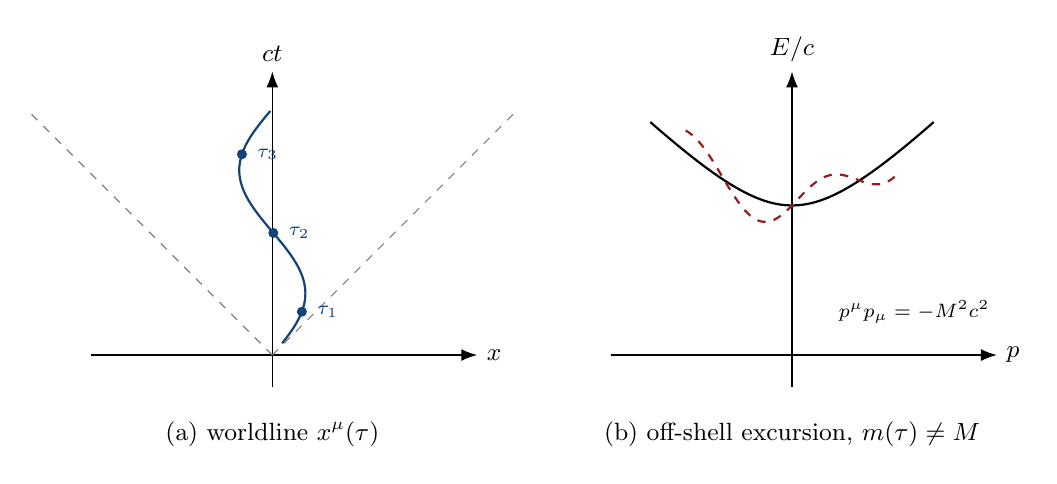
\begin{tikzpicture}[scale=1.0,>=Latex]
\begin{scope}
\draw[-{Latex[length=2mm]}] (-2.3,0) -- (2.6,0) node[right] {\small $x$};
\draw[-{Latex[length=2mm]}] (0,-0.4) -- (0,3.6) node[above] {\small $ct$};
\draw[gray,dashed] (0,0) -- (3.1,3.1);
\draw[gray,dashed] (0,0) -- (-3.1,3.1);
\draw[thick,shpblue,domain=0.15:3.1,samples=80,smooth]
   plot ({0.42*sin(115*\x)}, {\x});
\foreach \t/\lab in {0.55/{\tau_1},1.55/{\tau_2},2.55/{\tau_3}}{
   \pgfmathsetmacro{\xx}{0.42*sin(115*\t)}
   \filldraw[shpblue] (\xx,\t) circle (1.6pt);
   \node[shpblue,right] at (\xx+0.07,\t) {\scriptsize $\lab$};
}
\node at (0,-1.0) {\small (a) worldline $x^\mu(\tau)$};
\end{scope}
\begin{scope}[xshift=6.6cm]
\draw[-{Latex[length=2mm]}] (-2.3,0) -- (2.6,0) node[right] {\small $p$};
\draw[-{Latex[length=2mm]}] (0,-0.4) -- (0,3.6) node[above] {\small $E/c$};
\draw[thick,black,domain=-1.8:1.8,samples=80,smooth]
   plot(\x,{sqrt(1+\x*\x)+0.9});
\draw[thick,dashed,shpred,domain=-1.35:1.35,samples=80,smooth]
   plot(\x,{sqrt(1+\x*\x)+0.9+0.28*sin(210*\x)});
\node at (1.55,0.55) {\scriptsize $p^\mu p_\mu=-M^2c^2$};
\node at (0,-1.0) {\small (b) off-shell excursion, $m(\tau)\neq M$};
\end{scope}
\end{tikzpicture}
\caption{Schematic illustration of a single SHP event. (a)~The worldline
$x^\mu(\tau)$ is traced out as the invariant parameter $\tau$ increases; unlike
ordinary proper time, $\tau$ is external to the trajectory. (b)~In momentum
space, the on-shell locus $p^\mu p_\mu=-M^2c^2$ (solid curve) is only the
asymptotic/free value; during an interaction the instantaneous dynamical mass
$m(\tau)$, set by $p^\mu(\tau) p_\mu(\tau)=-m(\tau)^2c^2$, generically departs
from and later relaxes back toward it (dashed curve), as in
\eqref{eq:massformula}.}
\label{fig:worldline}
\end{figure}

\begin{figure}[htbp]
\centering
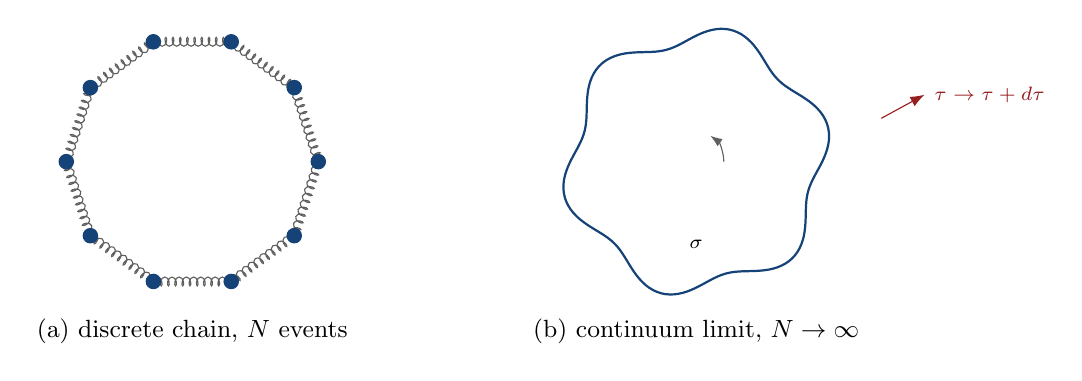
\begin{tikzpicture}[scale=1.0,>=Latex]
\begin{scope}
\foreach \i in {0,...,9}{
  \pgfmathsetmacro{\ang}{36*\i}
  \coordinate (P\i) at ({1.6*cos(\ang)},{1.6*sin(\ang)});
}
\foreach \i in {0,...,9}{
  \pgfmathtruncatemacro{\j}{mod(\i+1,10)}
  \draw[shpgray,decorate,decoration={coil,aspect=0.55,segment length=2.6pt,amplitude=1.6pt}]
     (P\i) -- (P\j);
}
\foreach \i in {0,...,9}{
  \filldraw[shpblue] (P\i) circle (2.6pt);
}
\node at (0,-2.15) {\small (a) discrete chain, $N$ events};
\end{scope}
\begin{scope}[xshift=6.4cm]
\draw[thick,shpblue,samples=200,smooth,domain=0:360]
   plot({(1.6+0.13*sin(6*\x))*cos(\x)},{(1.6+0.13*sin(6*\x))*sin(\x)});
\draw[-{Latex[length=1.8mm]},shpred] (2.35,0.55) -- (2.9,0.85);
\node[shpred,right] at (2.9,0.85) {\scriptsize $\tau\to\tau+d\tau$};
\node at (0,-1.05) {\scriptsize $\sigma$};
\draw[-{Latex[length=1.5mm]},shpgray] (0.35,0) arc (0:55:0.4);
\node at (0,-2.15) {\small (b) continuum limit, $N\to\infty$};
\end{scope}
\end{tikzpicture}
\caption{From a discrete chain to the SHP string. (a)~$N$ off-shell events
bound to their nearest neighbors by invariant-interval spring-like potentials,
\eqref{eq:chainK}; the steady solution is a rigidly rotating ring
(Section~\ref{sec:steady}). (b)~In the continuum limit the chain becomes a
smooth string $x^\mu(\sigma,\tau)$, with $\sigma$ labeling position along the
string and the single universal parameter $\tau$ evolving the entire
configuration, including the transverse oscillation modes of
Section~\ref{sec:modes}.}
\label{fig:chain}
\end{figure}


%############################################################################
\section{Comparison with the Nambu--Goto/Polyakov String}
\label{sec:comparison}
%############################################################################

\subsection{Constrained versus unconstrained construction}

The conventional relativistic string is defined by a reparametrization- and
Weyl-invariant action, most transparently the Polyakov form
$S\propto\int d^2\sigma\,\sqrt{-h}\,h^{ab}\partial_a X^\mu\partial_b X_\mu$,
in which the worldsheet metric $h_{ab}$ and coordinates $(\sigma^0,\sigma^1)$
are auxiliary and gauge, respectively. Physical states are extracted only
after imposing the Virasoro constraints -- the residual generators of
worldsheet reparametrizations -- as conditions on the state space; covariant
canonical quantization of this constrained system must then confront negative-norm
states associated with timelike oscillator modes, resolved either by fixing
light-cone gauge, by BRST quantization, or by the no-ghost theorem, all of
which are intimately tied to the existence of a critical spacetime dimension
($D=26$ for the bosonic string, $D=10$ for the superstring) at which the
worldsheet conformal anomaly cancels. In this setting, ``off-shell'' string
configurations are simply those that violate the Virasoro constraints -- a
gauge artifact to be projected away, not an independent physical freedom.

The SHP string of Section~\ref{sec:string} is built along an entirely
different route. There is no worldsheet reparametrization symmetry to gauge
fix and no Virasoro algebra to solve; $\tau$ is not a worldsheet coordinate
but the same universal, physical evolution parameter that appears already at
the level of the single event in Section~\ref{sec:single}, and the theory is
quantized by directly diagonalizing an unconstrained covariant Hamiltonian.
``Off-shell'' here means what it means for the point particle: the local
four-momentum of the string, at any given $\sigma$ and $\tau$, need not satisfy
a fixed mass-shell condition, and the composite mass $m$ of
\eqref{eq:massspectrum} is a genuinely dynamical output of the theory, not a
constraint eigenvalue.

\subsection{No critical dimension}

A direct consequence is that the SHP string requires no critical spacetime
dimension: because quantization proceeds by building positive-norm states
directly out of the positive-definite RMS eigenfunctions of
Section~\ref{sec:oscillator}, mode by mode, there are no negative-norm
oscillators to remove in the first place, and hence no conformal-anomaly
condition to satisfy by adjusting the target-space dimension. As Suleymanov,
Horwitz and Yahalom put it, in this framework ``there is no need for
additional dimensions'' \cite{SuleymanovHorwitzYahalom2017}: the construction
of Section~\ref{sec:string} is carried out directly in physical $3+1$
spacetime dimensions.

\subsection{A structural tension: reparametrization invariance versus off-shell freedom}
\label{sec:tension}

The price of this simplification is worth stating precisely, since it reflects
a structural, not merely technical, distinction between the two frameworks.
Frastai and Horwitz observed that the off-shell theory, viewed from the
Schwinger--Feynman path-integral perspective, does not admit a Hamiltonian
representation if it is required to be reparametrization invariant
\cite{FrastaiHorwitz1995}. The point is transparent already for a single free
particle: a reparametrization-invariant Lagrangian of the form
$\int ds\,\sqrt{\dot q^\mu\dot q_\mu}$ (dots denoting $d/ds$ for an arbitrary
parameter $s$) yields a canonical momentum
$p^\mu\propto \dot q^\mu/\sqrt{\dot q^\nu\dot q_\nu}$ that is automatically
homogeneous of degree zero in $\dot q^\mu$ and hence \emph{constant} along the
trajectory -- a necessarily on-shell quantity, since reparametrization
invariance forces the mass-shell condition to appear as a first-class
constraint rather than as a dynamical equation of motion. Gaining a genuine
dynamical mass therefore requires giving up manifest worldline (or worldsheet)
reparametrization invariance in favor of a genuinely Hamiltonian formulation
with a fixed, physical evolution parameter -- and vice versa. The SHP string
and the Nambu--Goto/Polyakov string sit at opposite poles of this trade-off:
the former keeps off-shell freedom at the price of reparametrization
invariance; the latter keeps reparametrization invariance at the price of
confining physical states to the mass shell.

\subsection{Origin of Regge-like behavior}

Both frameworks yield a mass-squared spectrum approximately linear in the
excitation (angular-momentum-like) quantum number, matching the qualitative
Regge phenomenology of hadron spectroscopy. In the Nambu--Goto/Polyakov
string this arises from an essentially geometric argument -- the area law of
the classical action together with the conformal-field-theoretic structure of
the quantum worldsheet -- whereas in the SHP string, as
\eqn{eq:massspectrum} makes explicit, it arises directly from summing
quantized relativistic-oscillator mode energies of an underlying lattice of
interacting events. The two constructions offer, in this sense, geometric and
dynamical explanations of the same qualitative phenomenon.

\begin{table}[htbp]
\centering
\small
\renewcommand{\arraystretch}{1.25}
\begin{tabular}{@{}>{\raggedright\arraybackslash}p{3.1cm}>{\raggedright\arraybackslash}p{3.9cm}>{\raggedright\arraybackslash}p{3.9cm}>{\raggedright\arraybackslash}p{3.9cm}@{}}
\toprule
& \textbf{SHP string} & \textbf{Nambu--Goto/Polyakov string} & \textbf{Pavši\v{c} unconstrained $p$-brane} \\
\midrule
Evolution parameter & Universal, physical $\tau$ (Sec.~\ref{sec:single}) & Worldsheet coordinate, gauge & Universal, physical $\tau$-type parameter \\
Constraint structure & None; genuinely Hamiltonian & Virasoro constraints (first class) & None in the unconstrained formulation \\
Mass-shell status & Dynamical, off-shell generically & Fixed by constraints (on-shell) & Dynamical, off-shell generically \\
Critical dimension & Not required & Required ($D=26$ bosonic, $D=10$ super) & Not required \\
Underlying degrees of freedom & Discrete lattice of off-shell events $\to$ continuum & Continuous embedding field $X^\mu(\sigma^a)$ & Single Stueckelberg-type point in membrane space $\mathcal M$ \\
Quantization route & Direct diagonalization onto positive-norm RMS eigenfunctions & Ladder operators; ghosts removed via gauge/BRST/no-ghost theorem & Field theory on $\mathcal M$; recovers Dirac--Nambu--Goto for a suitable field-space metric \\
Origin of Regge-like spectrum & Sum of quantized lattice-oscillator energies & Geometric area law / CFT central charge & Not the primary focus of the construction \\
\bottomrule
\end{tabular}
\caption{Structural comparison of the three extended-object frameworks
discussed in this paper. See Section~\ref{sec:comparison} for the SHP string
versus the standard string, and Section~\ref{sec:pavsic} for Pavši\v{c}'s
unconstrained $p$-branes.}
\label{tab:comparison}
\end{table}


%############################################################################
\section{A Parallel Programme: Pavši\v{c}'s Unconstrained $p$-Branes}
\label{sec:pavsic}
%############################################################################

\subsection{The Fock--Schwinger--Stueckelberg route to $p$-branes}

Independently of the Horwitz--Piron--Arshansky--Land line of development,
Matej Pavši\v{c} developed, from the early 1990s onward, an extensive
``unconstrained'' formulation of relativistic particle, string and $p$-brane
dynamics built around the same core Stueckelberg idea of an invariant
evolution parameter
\cite{Pavsic1991a,Pavsic1991b,Pavsic1993}. This programme generalizes the
Fock--Schwinger--Stueckelberg proper-time formalism directly to $p$-branes
\cite{PavsicPbranes1996}: rather than building the extended object bottom-up
from a lattice of interacting point events, as in Section~\ref{sec:string},
Pavši\v{c} introduces a \emph{membrane space} $\mathcal M$, the infinite-dimensional
space of all possible embeddings of a fixed $p$-brane into target spacetime,
and treats the brane's dynamics as that of a single Stueckelberg-type point
event moving through $\mathcal M$ with respect to a Poincar\'e- (or, in the
membrane-space generalization, diffeomorphism-) invariant evolution parameter.
Conventional $p$-brane configurations, subject to the usual Dirac--Nambu--Goto
constraints, appear in this scheme as particular stationary solutions of a
covariant Schr\"odinger-type equation on $\mathcal M$, recovered from the
unconstrained theory for a suitable choice of metric on the field space of
embeddings \cite{Pavsic1991a}.

\subsection{Common ground with SHP theory}

The two programmes share three structural commitments. First, both treat the
evolution parameter as ontologically prior to, and distinct from, coordinate
time, following Stueckelberg. Second, both allow the physical configuration --
a particle's mass in SHP theory, an entire brane embedding in Pavši\v{c}'s
theory -- to lie generically off the classical constraint surface, recovering
the constrained (on-shell) theory only as a special or asymptotic sector.
Third, both explicitly discuss the mechanism by which the usual
reparametrization-invariant, constrained brane actions are recovered from the
unconstrained theory in a suitable limit, echoing the structural tension
described in Section~\ref{sec:tension}.

\subsection{Points of divergence}

The two constructions differ sharply in method and ambition. The SHP string of
Section~\ref{sec:string} is built bottom-up, in the spirit of statistical or
many-body mechanics: a finite lattice of ordinary Stueckelberg point-events in
ordinary $D$-dimensional Minkowski space, interacting through nearest-neighbor
potentials, taken to a continuum limit. Pavši\v{c}'s brane-space construction
is built top-down and is considerably more geometrically ambitious in its
later development, embedding the unconstrained brane theory within a
Clifford-algebra ``polyvector'' formalism (``$C$-space''), in which points,
1-loops, 2-loops and higher multivectors are treated on a common footing and
related by generalized (``polydimensional'') rotations that can mix objects of
different grade. To the best of our knowledge, an explicit dictionary between
the two constructions -- for instance, exhibiting the SHP string's discrete
lattice of events as a specific point, or family of points, in Pavši\v{c}'s
membrane space $\mathcal M$ -- has not been worked out in the published
literature; the two should currently be regarded as complementary, independently
motivated routes to the same broad idea (an invariant evolution parameter for
extended objects) rather than as two presentations of a single theory.


%############################################################################
\section{Outlook: Toward Off-Shell Membranes in SHP Theory}
\label{sec:outlook}
%############################################################################

\begin{remark}[Scope of this section]
Everything in this section is a proposed generalization, not an established
result. Suleymanov, Horwitz and Yahalom explicitly identify the extension of
their construction beyond the string as a subject for future research
\cite{SuleymanovHorwitzYahalom2017}, and we were unable to locate a published
SHP-specific treatment of membranes or higher $p$-branes. What follows is
therefore offered as a natural, step-by-step generalization of
Section~\ref{sec:string}'s logic, together with an honest account of the new
difficulties it raises.
\end{remark}

\subsection{A two-parameter lattice}

The construction of Section~\ref{sec:discretechain} generalizes immediately,
at the level of writing down a Hamiltonian, to a two-dimensional lattice of
off-shell events $q_{(n_1,n_2)}^\mu(\tau)$, $n_1=1,\dots,N_1$,
$n_2=1,\dots,N_2$ (indices periodic in both directions, describing a closed
membrane of toroidal topology), coupled to nearest neighbors in each lattice
direction with, in general, independent stiffnesses $k_1,k_2$:
\begin{equation}
K=\sum_{n_1,n_2}\tfrac12 m\,\dot q_{(n_1,n_2)\mu}\dot q_{(n_1,n_2)}^{\ \mu}
+\sum_{n_1,n_2}\tfrac12 k_1\big(\Delta_1 q\big)_\mu\big(\Delta_1 q\big)^\mu
+\sum_{n_1,n_2}\tfrac12 k_2\big(\Delta_2 q\big)_\mu\big(\Delta_2 q\big)^\mu\,,
\label{eq:membraneK}
\end{equation}
where $\Delta_1q\equiv q_{(n_1+1,n_2)}-q_{(n_1,n_2)}$ and
$\Delta_2q\equiv q_{(n_1,n_2+1)}-q_{(n_1,n_2)}$. This is a direct, and entirely
standard, generalization of \eqref{eq:chainK} -- the covariant analogue of
passing from a one-dimensional chain to a two-dimensional lattice in ordinary
elasticity theory -- and its continuum limit, with surface mass density $\rho$
and tension densities $\eta_1,\eta_2$, is the covariant membrane wave equation
\begin{equation}
\rho\,\frac{\partial^2 x^\mu}{\partial\tau^2}
=\eta_1\frac{\partial^2 x^\mu}{\partial(\sigma^1)^2}+\eta_2\frac{\partial^2 x^\mu}{\partial(\sigma^2)^2}\,,
\label{eq:membranewave}
\end{equation}
the direct two-dimensional analogue of \eqn{eq:waveeq}. Assuming toroidal
boundary conditions, $x^\mu(\sigma^1,\sigma^2,\tau)$ admits a double Fourier
expansion in four independent real basis functions per mode pair
$(n_1,n_2)$ (the products of $\cos$ and $\sin$ in each of $\sigma^1,\sigma^2$),
each again satisfying, mode by mode, an independent covariant harmonic
oscillator equation in $\tau$ with dispersion relation
\begin{equation}
W_{n_1n_2}=\sqrt{\left(\frac{2\pi n_1}{L_1}\right)^2\frac{\eta_1}{\rho}
+\left(\frac{2\pi n_2}{L_2}\right)^2\frac{\eta_2}{\rho}}\,,
\label{eq:membranedispersion}
\end{equation}
the two-dimensional analogue of \eqn{eq:Knosc}. If, as seems plausible by
direct analogy, each such mode is again governed by (now four, rather than
two, independent copies of) the Arshansky--Horwitz relativistic oscillator
restricted to the RMS domain, the quantization strategy of
Section~\ref{sec:quantization} -- building the full membrane wavefunction as a
product of known, positive-norm single-mode RMS eigenfunctions -- should carry
over in its logical structure essentially unchanged.

\subsection{New difficulties in two dimensions}

At least three genuinely new issues, absent in the one-dimensional case, arise
at this point.

\emph{Existence and stability of a rigid steady solution.} The rotating-ring
equilibrium of Section~\ref{sec:steady} rested on the existence of a
configuration with equal, constant, spacelike nearest-neighbor intervals. In
two dimensions, requiring equal spacelike intervals along \emph{two}
independent lattice directions simultaneously, for a lattice folded into a
closed spacelike two-surface consistently embedded in Minkowski space, is a
substantially more constrained geometric problem, closer in spirit to the
simplicial (Regge-calculus-type) discretizations used in numerical general
relativity than to the simple planar ring of the string case. Whether such a
rigid steady solution exists, and is stable, for a general closed topology
remains open.

\emph{Density of modes and the mass spectrum.} In the one-dimensional string,
each integer $n$ labels exactly one mode, so the mode sum in
\eqref{eq:massspectrum} has a mode density independent of frequency. In two
dimensions the number of modes with $W_{n_1n_2}$ below a given cutoff grows
quadratically rather than linearly with the cutoff -- the same combinatorial
fact that distinguishes the thermodynamics of a vibrating membrane (or the
Debye theory of a two-dimensional solid, where the phonon density of states
grows linearly in frequency) from that of a vibrating string (constant density
of states). This is expected to alter both the character of the zero-point
sum and the detailed form of the mass-squared formula analogous to
\eqref{eq:massspectrum}; whether a clean Regge-type linear law survives, or is
replaced by a more intricate area/topology-dependent law, is an open
quantitative question that the string-case analysis alone does not settle.

\emph{Coupling to gauge fields.} In conventional string theory, the string
worldsheet couples naturally to a two-form (Kalb--Ramond) background field, the
antisymmetric-tensor generalization of the vector potential to which a point
particle couples. It is natural to conjecture that a continuous sheet of
charged off-shell events would source a two-index ``sheet current,'' and that
such a current could couple consistently to a $p$-form generalization of the
pre-Maxwell field of Section~\ref{sec:gauge}, in structural analogy with the
Kalb--Ramond coupling. We emphasize that this is a conjecture based on the
structural parallel, not a derived result, and working it out in detail is
beyond the scope of the present discussion.

\subsection{Curved backgrounds: SHPGR}

Independently of the extended-object programme reviewed here, SHP theory has
been embedded into a fully general-relativistic setting -- denoted SHPGR -- in
which the canonical Poisson-bracket structure of Section~\ref{sec:single} is
shown to remain valid, in a suitably covariant sense, on a general spacetime
manifold, providing the basis for a canonical quantum theory in curved
spacetime with the SHP potential appearing as a spacetime scalar mass
distribution \cite{Horwitz2019GR}. Combining this curved-background embedding
with the flat-space extended-object construction of Section~\ref{sec:string}
(or its outlook generalization above) is, as far as we are aware, an entirely
open and unexplored direction, potentially relevant to a covariant off-shell
treatment of gravitating extended sources such as cosmic strings.


%############################################################################
\section{Discussion}
\label{sec:discussion}
%############################################################################

Drawing the threads of this paper together: SHP off-shell dynamics supplies
(i)~a genuine additional universal parameter $\tau$, playing for relativistic
many-body dynamics the role Newtonian time plays non-relativistically, and
thereby resolving the tension identified by the Currie--Jordan--Sudarshan
no-interaction theorem for manifestly covariant interacting systems;
(ii)~a dynamical notion of mass, with well-defined mechanisms
(Section~\ref{sec:massstability}) by which the familiar on-shell theory is
recovered as a limit; (iii)~an associated five-dimensional pre-Maxwell gauge
structure, required by $\tau$-local gauge invariance and reducing to ordinary
Maxwell theory upon $\tau$-integration; and (iv), the theme of this paper, a
natural, Hamiltonian route to extended objects, realized concretely for the
relativistic string in Section~\ref{sec:string}. That construction is
structurally distinct from -- built on an unconstrained Hamiltonian formalism
rather than a reparametrization-invariant Lagrangian, and requiring no
critical spacetime dimension -- yet phenomenologically evocative of (through
its Regge-like mass spectrum) the standard Nambu--Goto/Polyakov string, and it
sits conceptually alongside Pavši\v{c}'s independently developed unconstrained
$p$-brane programme, which pursues a structurally different, top-down route to
the same broad idea. The extension of the SHP string construction proper to
membranes and higher $p$-branes remains open; Section~\ref{sec:outlook}
sketched a plausible route, together with the specific new difficulties --
rigidity of the steady solution, the altered density of modes, and the
possible coupling to higher-form generalizations of the pre-Maxwell field --
that any such extension will need to confront.

A recurring theme throughout is that off-shell-ness and reparametrization
invariance are, in a precise sense articulated in
Section~\ref{sec:tension}, mutually exclusive routes to relativistic covariance
for an extended object: one may have a dynamical mass-shell together with an
externally fixed evolution parameter, or a fixed mass-shell together with a
gauged worldline/worldsheet parametrization, but not, within either framework
reviewed here, both at once. Making this trade-off explicit is, we think, one
of the more useful things a comparison of these two traditions has to offer.


%############################################################################
\section{Conclusion}
\label{sec:conclusion}
%############################################################################

We have reviewed the Stueckelberg--Horwitz--Piron formalism for off-shell
relativistic dynamics, from the single event through the many-body and gauge
sectors, and traced its extension to space-time extended objects through the
explicit construction of a relativistic string as the continuum limit of a
covariant chain of off-shell events. This construction reproduces
phenomenologically familiar features of extended relativistic objects --
notably a Regge-like mass spectrum -- from a Hamiltonian, unconstrained
starting point that dispenses with the critical-dimension requirement of
covariant string quantization, at the structural cost of manifest worldsheet
reparametrization invariance. We situated this result relative to the
independently developed unconstrained $p$-brane programme of Pavši\v{c}, which
shares its Stueckelberg-type philosophy but not its bottom-up, lattice-based
method, and we outlined -- as an explicitly flagged, open direction -- how the
string construction might be generalized to membranes. The relation between
off-shell dynamics and extended objects is, on the evidence reviewed here,
still a comparatively young corner of the SHP research programme, with its
central results so far limited to the string; the generalizations sketched in
Section~\ref{sec:outlook}, and the still-unexplored combination with the
curved-background SHPGR formalism, suggest that this corner has considerably
more structure still to be uncovered.


%############################################################################
\appendix
\section{Verification of the Restricted Minkowski Space Parametrization}
\label{app:rms}
%############################################################################

We verify directly that the parametrization \eqref{eq:RMSparam},
\[
x^0=\rho\sin\theta\sinh\beta,\quad
x^1=\rho\sin\theta\cos\phi\cosh\beta,\quad
x^2=\rho\sin\theta\sin\phi\cosh\beta,\quad
x^3=\rho\cos\theta\,,
\]
gives an interval of fixed spacelike square $x^\mu x_\mu=\rho^2$ for the metric
signature $\eta_{\mu\nu}=\mathrm{diag}(-1,+1,+1,+1)$ used throughout this paper. Using
$\cosh^2\beta-\sinh^2\beta=1$ and $\cos^2\phi+\sin^2\phi=1$,
\begin{align}
x^\mu x_\mu&=-(x^0)^2+(x^1)^2+(x^2)^2+(x^3)^2\notag\\
&=-\rho^2\sin^2\theta\sinh^2\beta
+\rho^2\sin^2\theta\cosh^2\beta\big(\cos^2\phi+\sin^2\phi\big)
+\rho^2\cos^2\theta\notag\\
&=\rho^2\sin^2\theta\big(\cosh^2\beta-\sinh^2\beta\big)+\rho^2\cos^2\theta\notag\\
&=\rho^2\sin^2\theta+\rho^2\cos^2\theta=\rho^2\,,
\end{align}
confirming that $\rho$ is directly the invariant spacelike separation, and that
$(\theta,\phi,\beta)$ span the remaining directions on each fixed-$\rho$
hyperboloid sheet, consistently with its use in
Sections~\ref{sec:RMS}--\ref{sec:oscillator} as coordinates on the restricted
Minkowski space.


%############################################################################
%                                REFERENCES
%############################################################################
\clearpage
\begin{thebibliography}{99}

\bibitem{Fock1937}
V.~Fock, ``Die Eigenzeit in der klassischen und in der Quantenmechanik,''
\textit{Phys. Z. Sowjetunion} \textbf{12}, 404 (1937).

\bibitem{Stueckelberg1941a}
E.~C.~G.~Stueckelberg, ``La signification du temps propre en m\'ecanique
ondulatoire,'' \textit{Helv. Phys. Acta} \textbf{14}, 372 (1941).

\bibitem{Stueckelberg1941b}
E.~C.~G.~Stueckelberg, ``Remarque \`a propos de la cr\'eation de paires de
particules en th\'eorie de relativit\'e,'' \textit{Helv. Phys. Acta}
\textbf{14}, 585 (1941).

\bibitem{Stueckelberg1942}
E.~C.~G.~Stueckelberg, \textit{Helv. Phys. Acta} \textbf{15}, 23 (1942).

\bibitem{CurrieJordanSudarshan1963}
D.~G.~Currie, T.~F.~Jordan, and E.~C.~G.~Sudarshan, ``Relativistic Invariance
and Hamiltonian Theories of Interacting Particles,'' \textit{Rev. Mod. Phys.}
\textbf{35}, 350 (1963).

\bibitem{HorwitzPiron1973}
L.~P.~Horwitz and C.~Piron, ``Relativistic dynamics,'' \textit{Helv. Phys.
Acta} \textbf{46}, 316 (1973).

\bibitem{NewtonWigner1949}
T.~D.~Newton and E.~P.~Wigner, ``Localized States for Elementary Systems,''
\textit{Rev. Mod. Phys.} \textbf{21}, 400 (1949).

\bibitem{Horwitz2015}
L.~P.~Horwitz, \textit{Relativistic Quantum Mechanics}, Fundamental Theories
of Physics Vol.~180 (Springer, Dordrecht, 2015).

\bibitem{HorwitzArshanskyElitzur1988}
L.~P.~Horwitz, R.~I.~Arshansky, and A.~C.~Elitzur, ``On the two aspects of
time: The distinction and its implications,'' \textit{Found. Phys.}
\textbf{18}, 1159 (1988).

\bibitem{ArshanskyHorwitz1989}
R.~I.~Arshansky and L.~P.~Horwitz, ``The quantum relativistic two-body bound
state. I. The spectrum,'' \textit{J. Math. Phys.} \textbf{30}, 66 (1989).

\bibitem{Zmuidzinas1966}
J.~Zmuidzinas, ``Unitary representations of the Lorentz group on 4-vector
manifolds,'' \textit{J. Math. Phys.} \textbf{7}, 764 (1966).

\bibitem{SaadHorwitzArshansky1989}
D.~Saad, L.~P.~Horwitz, and R.~I.~Arshansky, ``Off-shell electromagnetism in
manifestly covariant relativistic quantum mechanics,'' \textit{Found. Phys.}
\textbf{19}, 1125 (1989).

\bibitem{LandHorwitz1991}
M.~C.~Land and L.~P.~Horwitz, ``Green's functions for off-shell
electromagnetism and spacelike correlations,'' \textit{Found. Phys.}
\textbf{21}, 299 (1991).

\bibitem{Land1997}
M.~C.~Land, ``Particles and events in classical off-shell electrodynamics,''
\textit{Found. Phys.} \textbf{27}, 19 (1997).

\bibitem{FrastaiHorwitz1995}
J.~Frastai and L.~P.~Horwitz, ``Off-Shell Fields and Pauli--Villars
Regularization,'' \textit{Found. Phys.} \textbf{25}, 1495 (1995).

\bibitem{AharonovichHorwitz2011}
I.~Aharonovich and L.~Horwitz, ``Radiation-reaction in classical off-shell
electrodynamics. I. The above mass-shell case,'' \textit{J. Math. Phys.}
\textbf{53}, 032902 (2011).

\bibitem{BurakovskyHorwitzSchieve1996}
L.~Burakovsky, L.~Horwitz, and W.~C.~Schieve, ``A New Relativistic High
Temperature Bose--Einstein Condensation,'' \textit{Phys. Rev. D} \textbf{54},
4029 (1996).

\bibitem{HorwitzStrangeAttractor2004}
L.~P.~Horwitz \textit{et al.}, ``Could the classical relativistic electron be
a strange attractor?,'' \textit{Discrete Dyn. Nat. Soc.} \textbf{2004}, 237
(2004).

\bibitem{SuleymanovHorwitzYahalom2017}
M.~Suleymanov, L.~Horwitz, and A.~Yahalom, ``Second quantization of a
covariant relativistic spacetime string in Steuckelberg--Horwitz--Piron
theory,'' \textit{Front. Phys.} \textbf{12}, 121103 (2017); arXiv:1612.04193.

\bibitem{Polchinski1998}
J.~Polchinski, \textit{String Theory, Vol.~1: An Introduction to the Bosonic
String} (Cambridge University Press, Cambridge, 1998).

\bibitem{Pavsic1991a}
M.~Pavši\v{c}, ``On the interpretation of the relativistic quantum mechanics
with invariant evolution parameter,'' \textit{Found. Phys.} \textbf{21}, 1005
(1991).

\bibitem{Pavsic1991b}
M.~Pavši\v{c}, ``Relativistic quantum mechanics and quantum field theory with
invariant evolution parameter,'' \textit{Nuovo Cimento A} \textbf{104}, 1337
(1991).

\bibitem{Pavsic1993}
M.~Pavši\v{c}, ``The role of the invariant evolution parameter in
relativistic particles and strings,'' \textit{Do\u{g}a, Turkish J. Phys.}
\textbf{17}, 768 (1993).

\bibitem{PavsicPbranes1996}
M.~Pavši\v{c}, ``Fock--Schwinger proper time formalism for $p$-branes,''
arXiv:hep-th/9612151.

\bibitem{Horwitz2019GR}
L.~P.~Horwitz, ``An Elementary Canonical Classical and Quantum Dynamics for
General Relativity,'' \textit{Eur. Phys. J. Plus} \textbf{134}, 313 (2019);
arXiv:1810.09248.

\end{thebibliography}

\end{document}
